\documentclass[12pt,letterpaper]{article}

% Evidencia: GA4-220501095-AA3-EV01
% Compilar con LaTeX Workshop o: latexmk -pdf GA4-220501095-AA3-EV01.tex
% El contenido usa caracteres ASCII para evitar problemas de codificacion.

\usepackage[spanish,es-nodecimaldot,shorthands=off]{babel}
\usepackage[T1]{fontenc}
\usepackage[utf8]{inputenc}
\usepackage{lmodern}
\usepackage{geometry}
\usepackage{setspace}
\usepackage{array}
\usepackage{longtable}
\usepackage{enumitem}
\usepackage{xcolor}
\usepackage{titlesec}
\usepackage{fancyhdr}
\usepackage{graphicx}
\usepackage{pdflscape}
\usepackage{hyperref}

% ==================== DATOS CONFIGURABLES ====================
\newcommand{\institucion}{Servicio Nacional de Aprendizaje -- SENA}
\newcommand{\programa}{Analisis y Desarrollo de Software}
\newcommand{\tituloTrabajo}{Mapa conceptual: Identificacion y caracterizacion de los componentes del ciclo de vida del software}
\newcommand{\codigoEvidencia}{GA4-220501095-AA3-EV01}
\newcommand{\aprendiz}{Kevin Andres Granados Daza}
\newcommand{\instructor}{[Jesus Ramirez]}
\newcommand{\ficha}{[3389015]}
\newcommand{\ciudad}{Bogota D. C.}
\newcommand{\fechaEntrega}{[25 de septiembre de 2026]}
% ==============================================================

\geometry{top=2.54cm,bottom=2.54cm,left=2.54cm,right=2.54cm}
\onehalfspacing
\setlength{\parindent}{1.27cm}
\setlength{\parskip}{0pt}
\setlength{\headheight}{15pt}

\pagestyle{fancy}
\fancyhf{}
\fancyhead[L]{\codigoEvidencia}
\fancyhead[R]{\thepage}
\renewcommand{\headrulewidth}{0pt}

\titleformat{\section}{\normalfont\Large\bfseries\centering}{\thesection.}{0.5em}{}
\titleformat{\subsection}{\normalfont\large\bfseries}{\thesubsection.}{0.5em}{}

\begin{document}

\begin{titlepage}
    \centering
    \vspace*{2.5cm}
    {\Large \tituloTrabajo\par}
    \vfill
    {\large \aprendiz\par}
    \vspace{1.5cm}
    {\large \institucion\par}
    {\large \programa\par}
    \vspace{1cm}
    {\large Evidencia: \codigoEvidencia\par}
    \vspace{1cm}
    {\large Instructor: \instructor\par}
    {\large Ficha: \ficha\par}
    \vfill
    {\large \ciudad\par}
    {\large \fechaEntrega\par}
\end{titlepage}

\section{Introduccion}

El ciclo de vida del software comprende el conjunto de procesos, actividades y tareas que se realizan para planear, desarrollar, probar, entregar, operar, mantener y retirar una solucion informatica. Su importancia radica en que permite organizar el trabajo de forma ordenada y controlar que las necesidades de los usuarios se transformen en un producto de calidad.

Cada etapa del ciclo de vida tiene objetivos, actividades y entregables propios. La planificacion permite definir el problema, el alcance y los recursos; el analisis identifica los requisitos; el diseno define la solucion; el desarrollo convierte el diseno en codigo; las pruebas verifican el funcionamiento; el despliegue pone el sistema a disposicion de los usuarios; y el mantenimiento permite corregir, adaptar y mejorar la aplicacion despues de su entrega.

El presente documento contiene un mapa conceptual que identifica y caracteriza los componentes principales del ciclo de vida del software. El mapa utiliza enlaces y palabras de relacion para mostrar la logica entre las etapas, los procesos transversales y el caracter iterativo del mantenimiento.

\section{Mapa conceptual del ciclo de vida del software}

A continuacion, se presenta el mapa conceptual elaborado mediante una herramienta TIC. El mapa organiza el ciclo de vida del software como concepto central y relaciona las etapas de planificacion, requisitos y analisis, diseno, desarrollo, pruebas, despliegue, operacion, mantenimiento y retiro. Tambien incorpora los procesos transversales que apoyan todas las fases del ciclo de vida.

% INSTRUCCION:
% Guarda la imagen exportada desde Draw.io con este nombre exacto:
% mapa_conceptual_ciclo_vida_software.png
% Ubicala en la misma carpeta que este archivo .tex.

\begin{figure}[htbp]
    \centering
    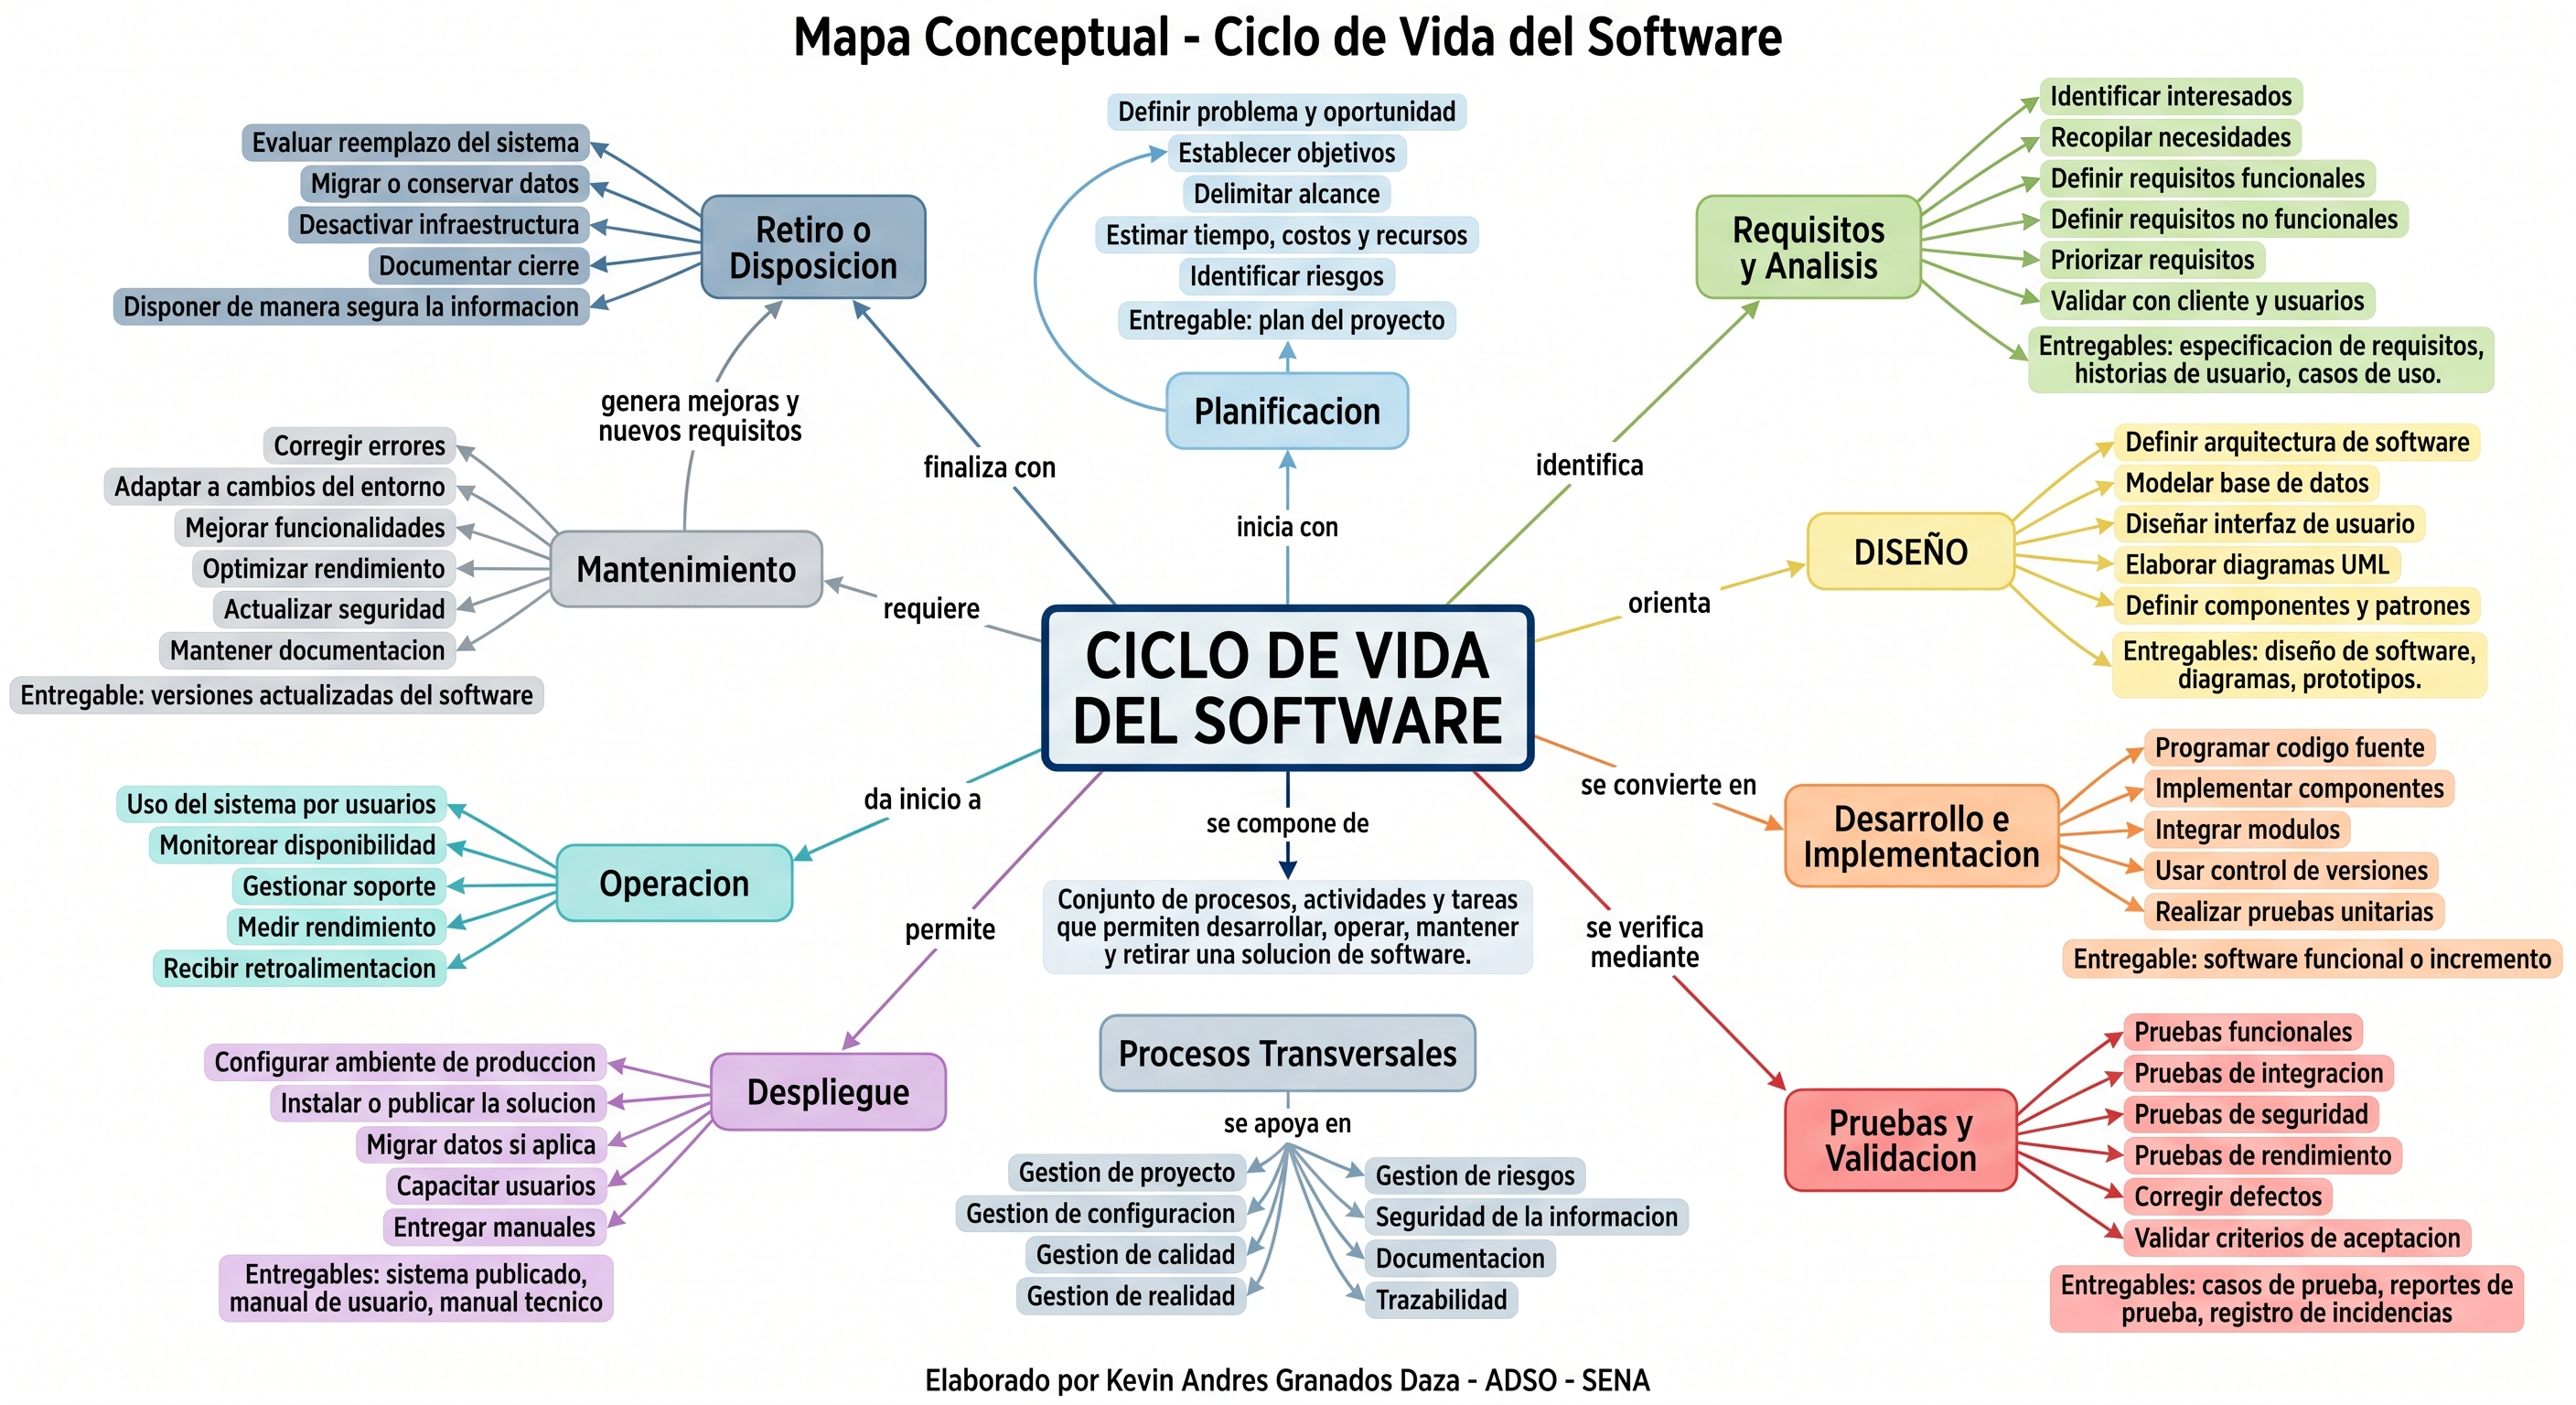
\includegraphics[width=1\textwidth]{mapa_conceptual_ciclo_vida_software.jpg}
    \caption{Mapa conceptual de los componentes del ciclo de vida del software.}
    \label{fig:mapa-ciclo-vida-software}
\end{figure}


Como se observa en la Figura~\ref{fig:mapa-ciclo-vida-software}, el ciclo de vida del software inicia con la planificacion y continua con la identificacion de requisitos, el diseno de la solucion, la implementacion, las pruebas y el despliegue. Despues de la entrega, el sistema entra en operacion y mantenimiento. Esta ultima etapa puede generar correcciones, mejoras o nuevos requisitos, por lo que retroalimenta la planificacion y permite iniciar nuevas iteraciones del proceso.

\section{Caracterizacion de los componentes}

\begin{longtable}{|p{3.5cm}|p{5.5cm}|p{5.6cm}|}
\hline
\textbf{Componente} & \textbf{Caracterizacion} & \textbf{Productos o entregables principales} \\
\hline
\endfirsthead
\hline
\textbf{Componente} & \textbf{Caracterizacion} & \textbf{Productos o entregables principales} \\
\hline
\endhead
\hline
\endfoot
\hline
\endlastfoot

Planificacion & Define el problema, los objetivos, el alcance, los recursos, el tiempo, los costos y los riesgos del proyecto. & Plan de proyecto, cronograma, estimacion de recursos, alcance y registro de riesgos. \\
\hline

Requisitos y analisis & Identifica las necesidades de interesados y usuarios; define requisitos funcionales, no funcionales y reglas de negocio. & Especificacion de requisitos, historias de usuario, casos de uso y criterios de aceptacion. \\
\hline

Diseno & Establece como se construira la solucion mediante arquitectura, modelos, interfaces, base de datos y componentes. & Diagramas UML, diagramas entidad-relacion, prototipos, diseno de base de datos y arquitectura de software. \\
\hline

Desarrollo e implementacion & Convierte el diseno en codigo fuente mediante la construccion e integracion de los modulos de software. & Codigo fuente, configuracion del proyecto, versiones y componentes funcionales. \\
\hline

Pruebas y validacion & Comprueba que el sistema cumpla los requisitos y que los defectos sean identificados y corregidos. & Casos de prueba, reportes de prueba, registro de incidencias y evidencias de validacion. \\
\hline

Despliegue & Publica o instala el sistema en un ambiente donde pueda ser utilizado por sus usuarios. & Sistema instalado o publicado, manual de usuario, manual tecnico y configuracion de produccion. \\
\hline

Operacion & Corresponde al uso real del sistema, al soporte inicial y al monitoreo de su disponibilidad y rendimiento. & Registro de uso, solicitudes de soporte, indicadores y retroalimentacion de usuarios. \\
\hline

Mantenimiento & Corrige errores, adapta el sistema a cambios, mejora funcionalidades y actualiza medidas de seguridad. & Versiones actualizadas, correcciones, mejoras, documentacion actualizada y registro de cambios. \\
\hline

Retiro o disposicion & Evalua el cierre, reemplazo o desactivacion del sistema cuando ya no cumple las necesidades organizacionales. & Plan de retiro, migracion o conservacion de datos, cierre tecnico y desactivacion de infraestructura. \\
\hline

Procesos transversales & Actividades que apoyan todas las fases, como calidad, configuracion, documentacion, riesgos, seguridad y trazabilidad. & Plan de calidad, repositorio de codigo, matriz de trazabilidad, controles de seguridad y documentos del proyecto. \\
\hline
\end{longtable}

\section{Conceptos clave identificados}

El mapa conceptual se estructura alrededor de conceptos clave que permiten comprender la relacion entre las etapas del ciclo de vida del software:

\begin{itemize}[leftmargin=1.2cm]
    \item \textbf{Proceso:} conjunto organizado de actividades que persigue un objetivo dentro del ciclo de vida.
    \item \textbf{Actividad:} conjunto de tareas relacionadas que producen un resultado verificable.
    \item \textbf{Tarea:} accion concreta realizada por una persona o equipo, por ejemplo definir un requisito o ejecutar una prueba.
    \item \textbf{Requisito:} necesidad, capacidad o condicion que debe cumplir el sistema.
    \item \textbf{Entregable:} producto tangible generado durante una etapa, como un diagrama, documento, codigo, manual o reporte.
    \item \textbf{Validacion:} comprobacion de que el sistema satisface las necesidades del usuario o cliente.
    \item \textbf{Trazabilidad:} capacidad para relacionar un requisito con su diseno, implementacion, prueba y resultado.
    \item \textbf{Mantenimiento:} conjunto de acciones posteriores a la entrega que permiten corregir, adaptar o mejorar el software.
    \item \textbf{Iteracion:} repeticion controlada de etapas del ciclo de vida para incorporar cambios o nuevas funcionalidades.
\end{itemize}

\section{Relacion con el proyecto de software}

El ciclo de vida del software se puede aplicar al Sistema de Gestion de Citas SAC. Durante la planificacion se define la necesidad de centralizar la administracion de horarios y citas. En la etapa de requisitos se identifican funciones como registro de usuarios, consulta de disponibilidad, agendamiento, cancelacion, reprogramacion y gestion administrativa.

En el diseno se elaboran los diagramas de casos de uso, clases, actividad, entidad-relacion, componentes y despliegue. En el desarrollo se construye el frontend web, la API REST, los servicios de negocio y la base de datos. Posteriormente se ejecutan pruebas para comprobar que un horario no pueda tener mas de una cita activa y que solo un administrador pueda gestionar disponibilidad.

Finalmente, durante el despliegue se publica la aplicacion en un servidor o servicio en la nube. En operacion y mantenimiento se recopila retroalimentacion de usuarios, se corrigen defectos y se agregan mejoras, como recordatorios o nuevos reportes. Esto demuestra que el ciclo de vida no termina con la primera entrega, sino que continua mientras el sistema siga siendo utilizado.

\section{Conclusiones}

El ciclo de vida del software permite organizar el desarrollo de una solucion desde la identificacion de una necesidad hasta la entrega, operacion, mantenimiento y retiro del sistema. Cada componente cumple una funcion especifica y genera entregables que ayudan a controlar el avance del proyecto.

El mapa conceptual elaborado permite identificar que las fases de planificacion, requisitos, diseno, desarrollo, pruebas, despliegue, operacion y mantenimiento se encuentran relacionadas. Ademas, los procesos transversales de calidad, seguridad, documentacion, gestion de riesgos y trazabilidad apoyan todo el ciclo de vida y contribuyen a mejorar el resultado final.

Tambien se reconoce que el ciclo de vida del software es iterativo. El mantenimiento genera correcciones, adaptaciones y nuevas necesidades que pueden iniciar nuevamente actividades de planificacion, analisis, diseno y desarrollo. Esta retroalimentacion permite que el software evolucione de acuerdo con los cambios del entorno y las necesidades de sus usuarios.

En conclusion, aplicar un ciclo de vida organizado facilita la construccion de software de mayor calidad. Para el Sistema de Gestion de Citas SAC, cada etapa permite transformar los requisitos de usuarios y administradores en una aplicacion funcional, verificable, mantenible y preparada para futuras mejoras.

\end{document}
